While carrying out the survey of radiation equipment and installation, the permissible dose limits for radiation workers and members of the public should be kept in mind. The weekly limit for radiation workers and members of the public is 40mR and 2mR, respectively.
\subsection{Leakage measurement of teletherapy Unit}
\begin{figure}[H]
    \centering
    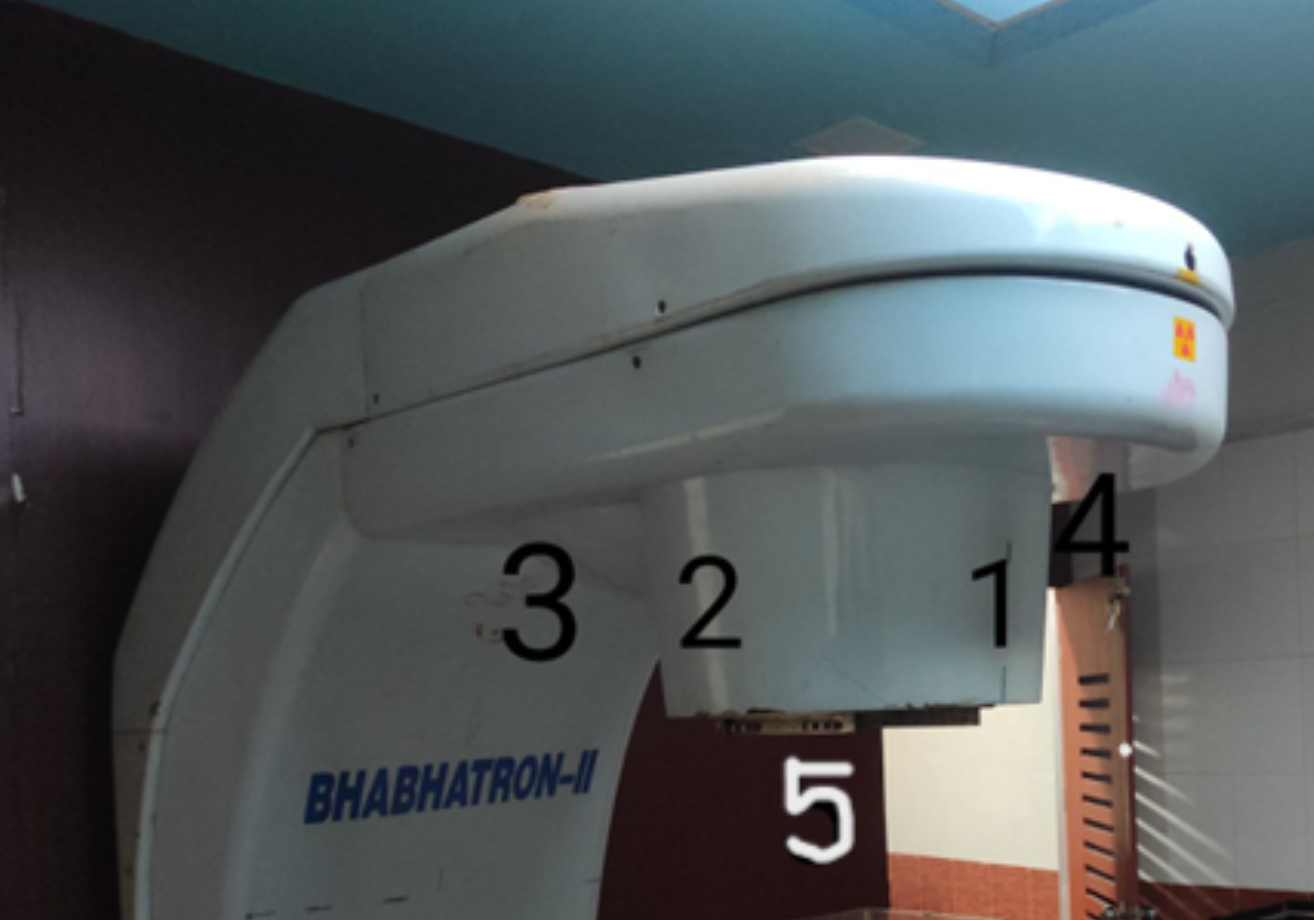
\includegraphics[width=0.7\textwidth]{Figures/Apparatus/TeleTherapyUnit.png}
    \caption{Gantry head of Teletherapy unit}
\end{figure}

\begin{figure}[H]
    \centering
    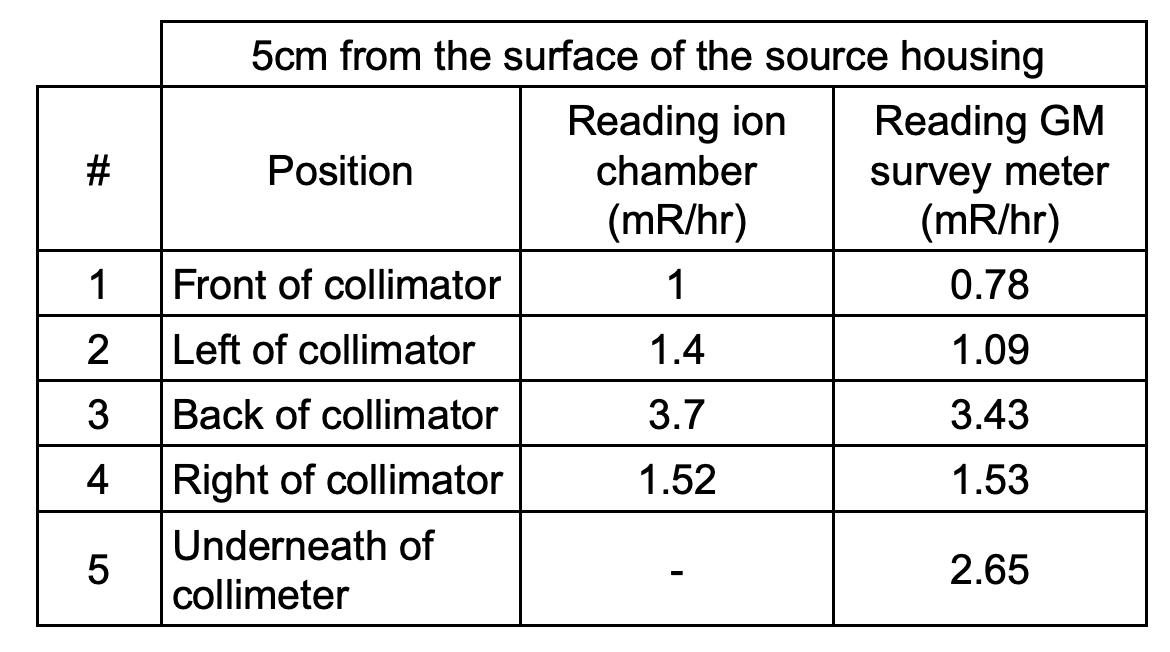
\includegraphics[width=0.7\textwidth]{Figures/Experimental data/LeakageMeasurmentBhabatron.png}
\end{figure}
\begin{figure}[H]
    \centering
    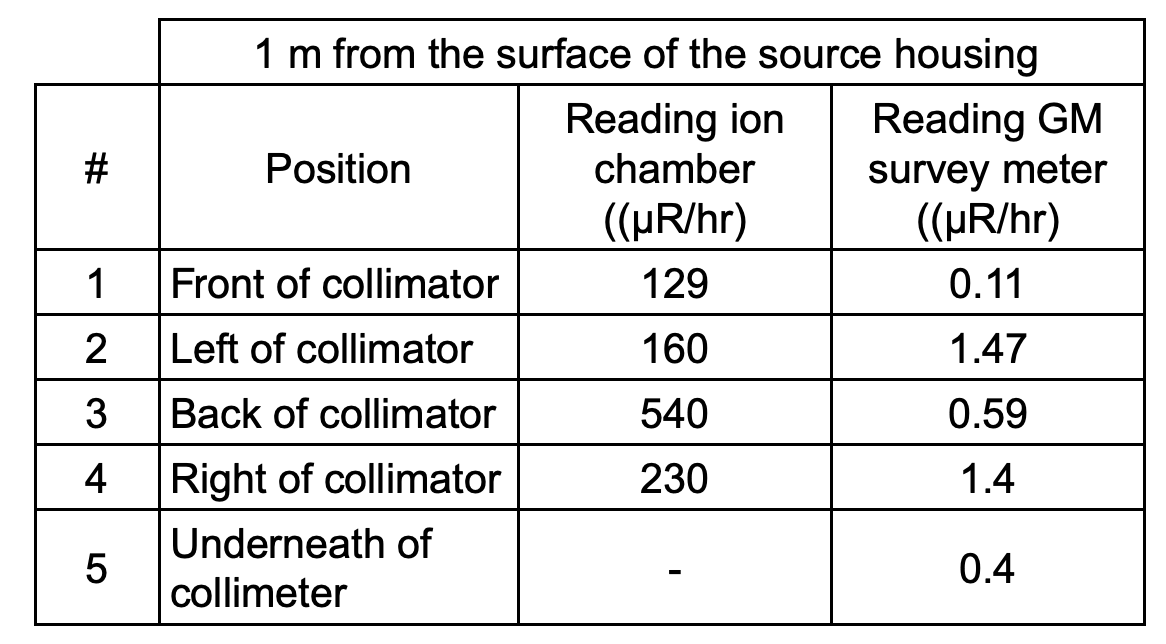
\includegraphics[width=0.7\textwidth]{Figures/Experimental data/LeakageMeasurmentBhabatron2.png}
\end{figure}

\begin{figure}[H]
    \centering
    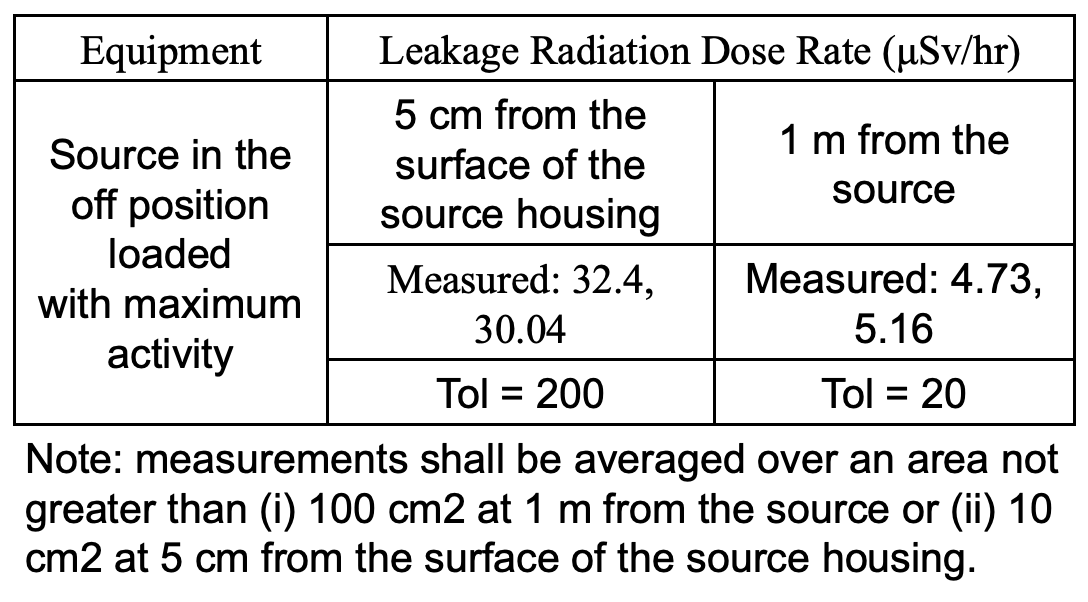
\includegraphics[width=0.7\textwidth]{Figures/Experimental data/LeakageMeasurmentBhabatron3.png}
\end{figure}

\subsection{Leakage measurement of Brachytherapy Unit}
Brachytherapy unit used Ir-192 source which is having current activity of 8.281 Ci. The source is kept inside the safe housing when not in use. The leakage measurement is carried out using a survey meter around the safe housing of the brachytherapy unit.
\begin{figure}[H]
    \centering
    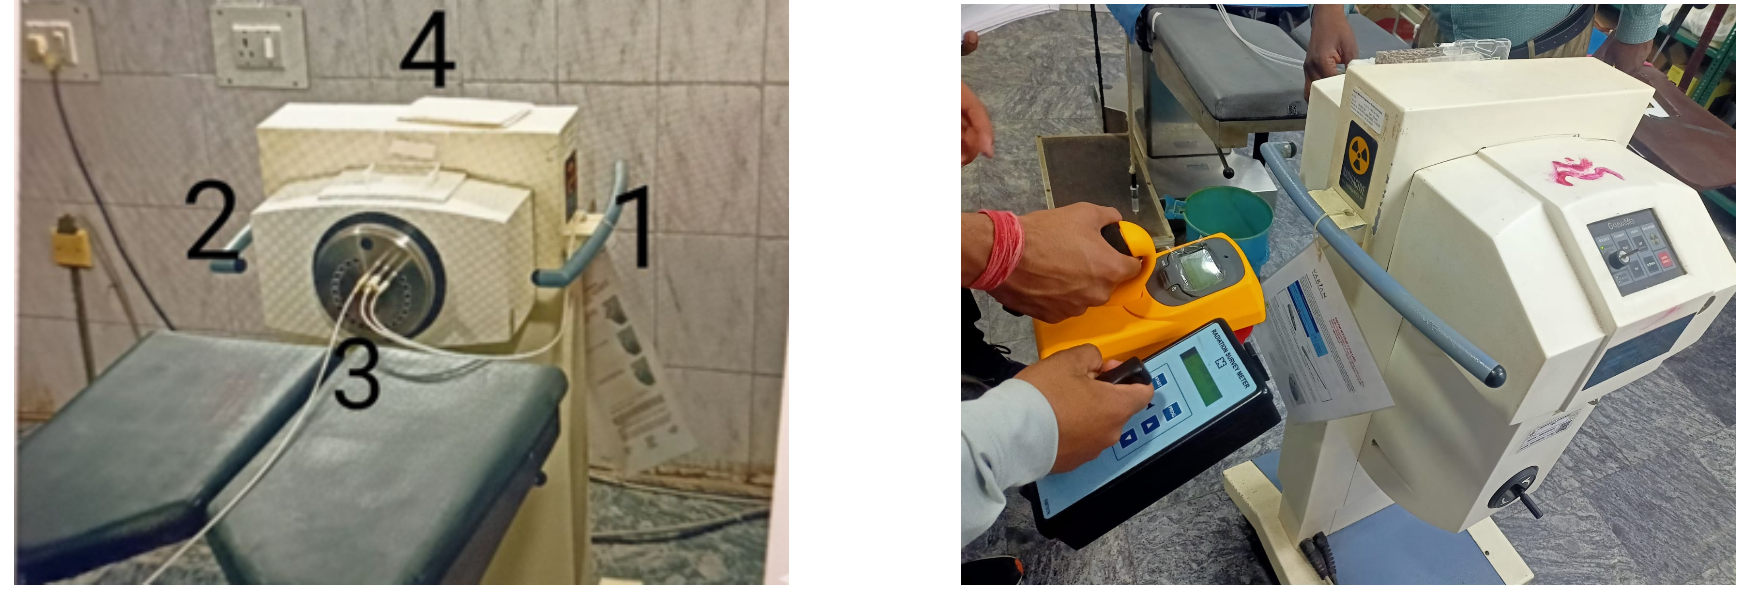
\includegraphics[width=0.7\textwidth]{Figures/Apparatus/Brachy.png}
    \caption{Brachytherapy unit}
\end{figure}
\begin{figure}[H]
    \centering
    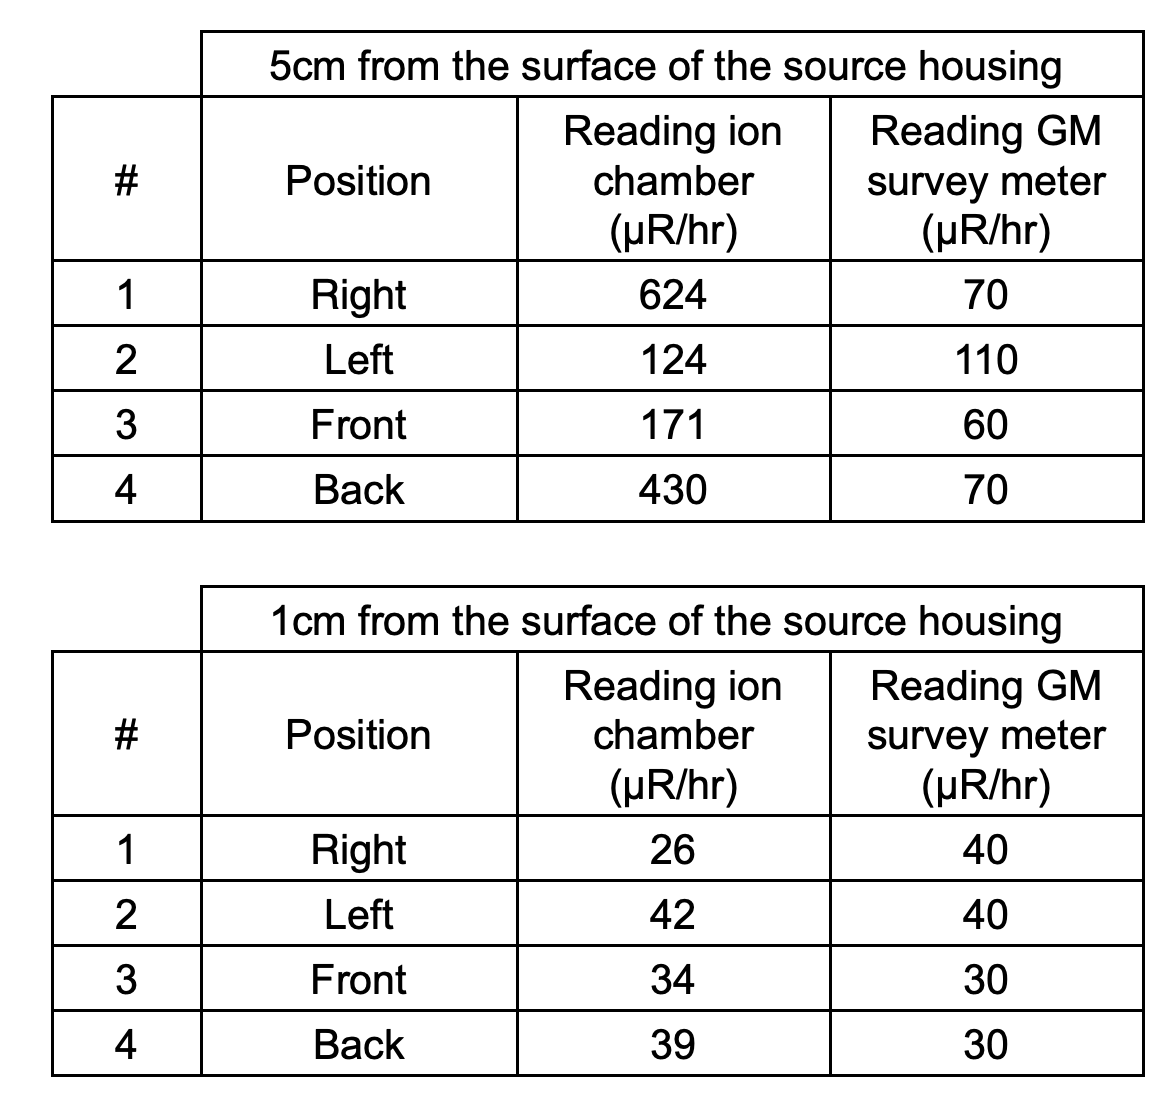
\includegraphics[width=0.7\textwidth]{Figures/Experimental data/BrachyDataLeakage.png}
\end{figure}
\begin{figure}[H]
    \centering
    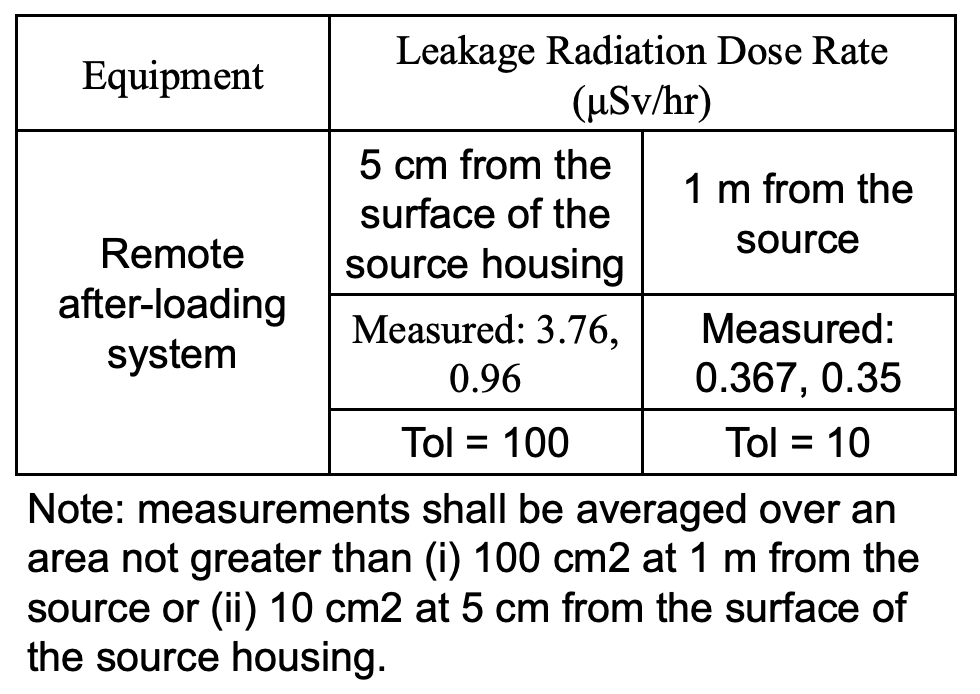
\includegraphics[width=0.6\textwidth]{Figures/Experimental data/BrachyDataLeakage2.png}
\end{figure}

\subsection{Survey of teletherapy} 
The survey of teletherapy unit is carried out using a survey meter around the teletherapy unit in the treatment room. The readings are tabulated below:
\begin{figure}[H]
    \centering
    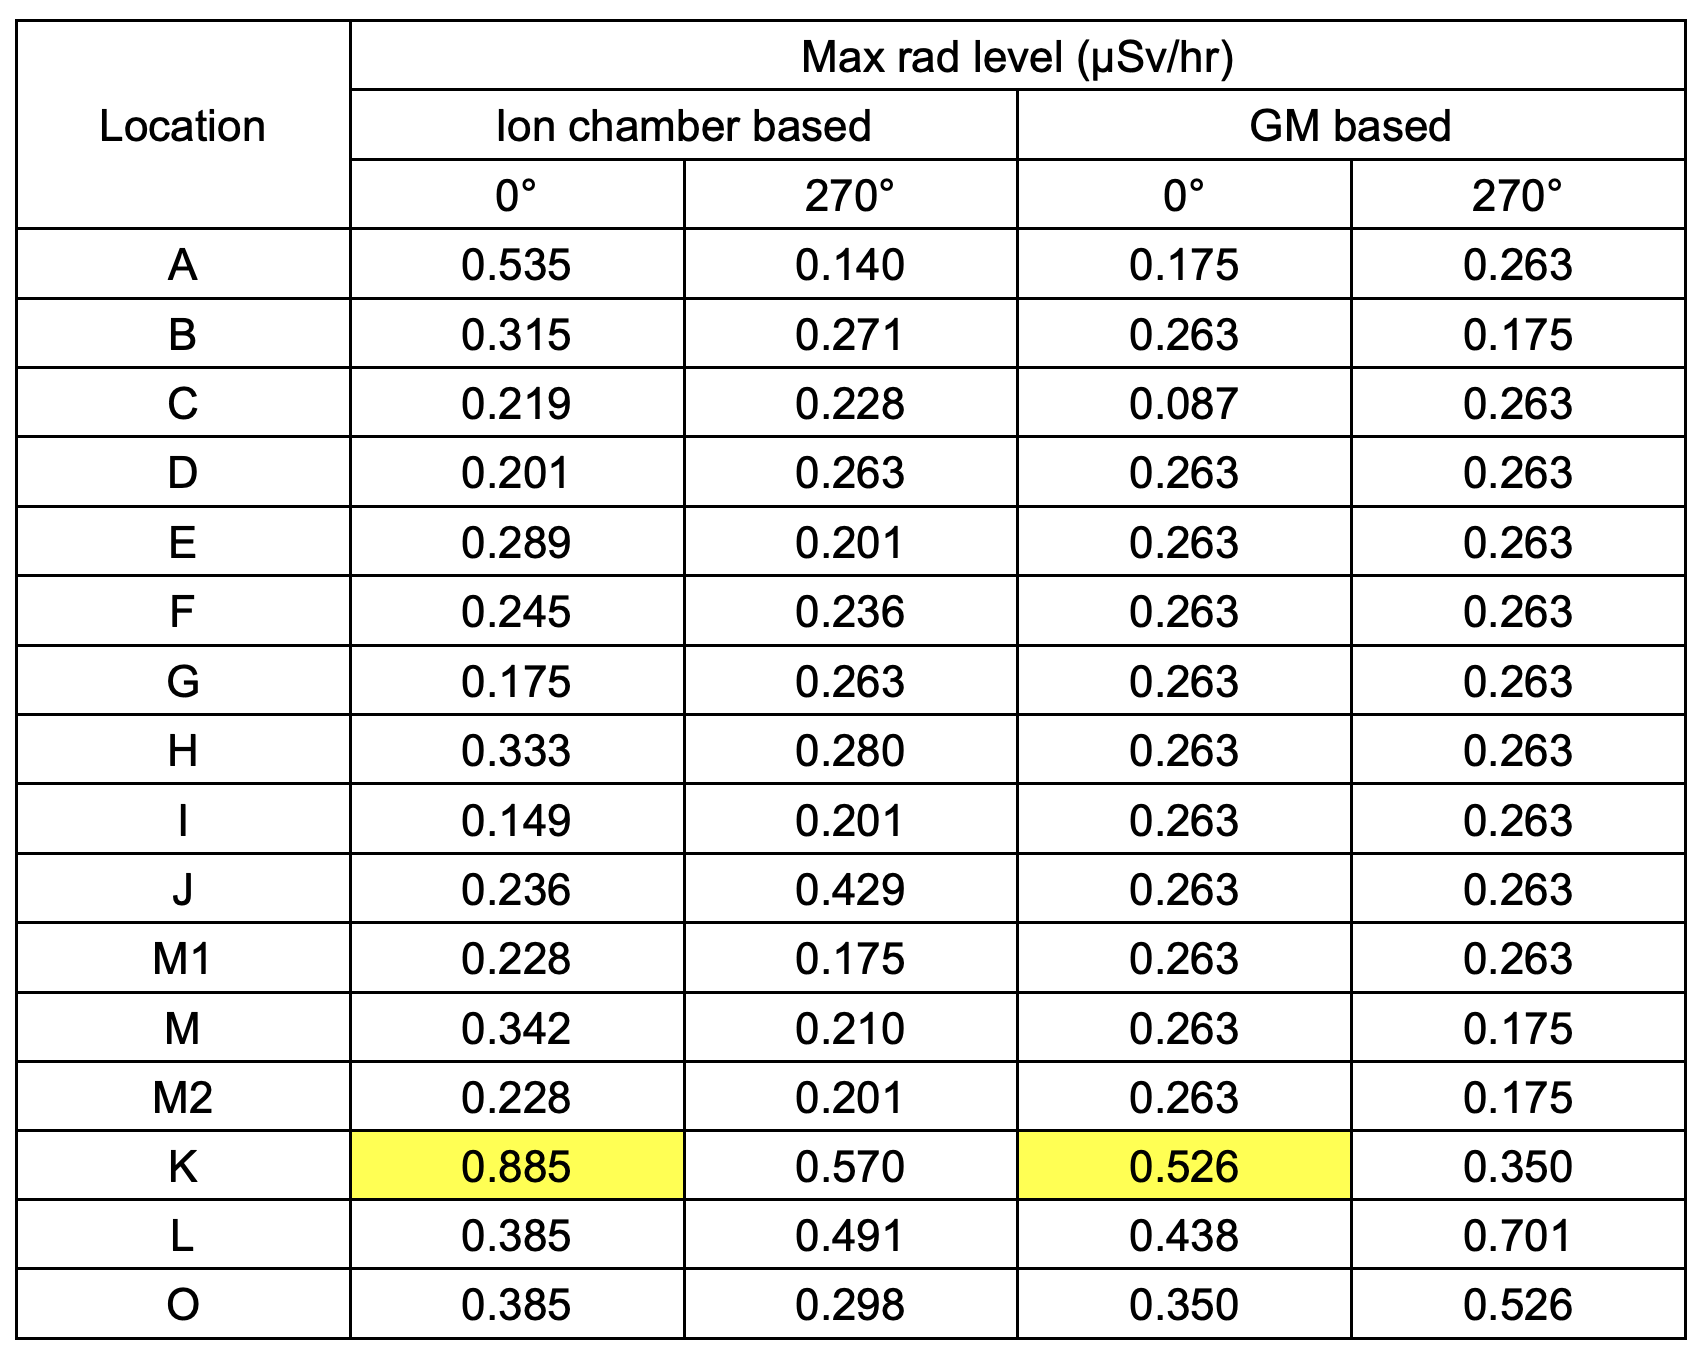
\includegraphics[width=0.7\textwidth]{Figures/Experimental data/SurveyofTeletherapy.png}
\end{figure}
\begin{figure}[H]
    \centering
    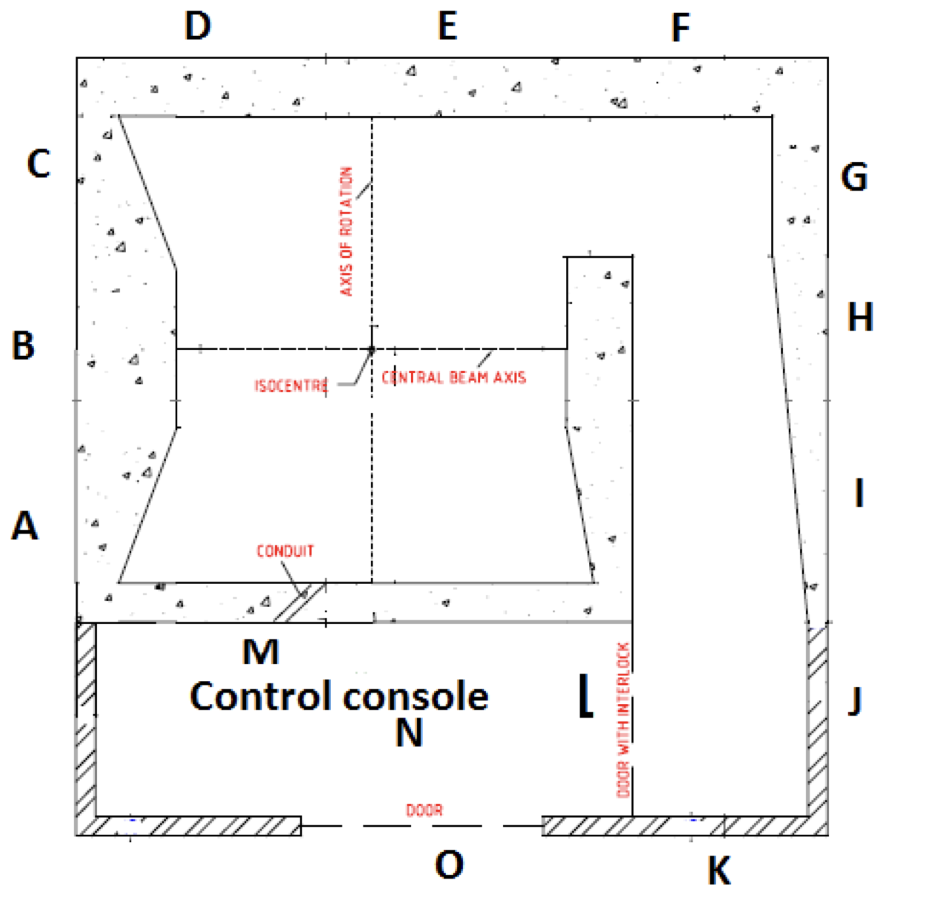
\includegraphics[width=0.4\textwidth]{Figures/Experimental data/LayoutofTeletherapy.png}
    \caption{Layout of teletherapy unit in treatment room}
\end{figure}
\subsubsection{Weekly Time Averaged Dose-Equivalent Rate}
If $R_w$ is the TADR averaged over a 40 hour week, it can be derived that \cite{IAEA_SafetyReport47_2006} :

\begin{equation}
R_W = \mathrm{IDR} \times \frac{WU}{\mathrm{DR}_0} 
\label{TADR}
\end{equation}


\begin{tabular}{ll}
$R_w$ & is the TADR averaged over one week, in $\mathrm{Sv}\cdot\mathrm{week}^{-1}$; \\
IDR & is instantaneous dose-equivalent rate in $\mathrm{Sv}\cdot\mathrm{h}^{-1}$ when the machine is operating at the dose output rate \\
 & $\mathrm{DR}_0$; \\
$W$ & is the weekly workload defined at 1 m in Gy; $= 1.5 \times 10^5 \, \mathrm{cGy/week} $ \\
$U$ & is the use factor (=1 for secondary barriers or the maze entrance);\\
$\mathrm{DR}_0$ & is the dose output rate at 1 m, in $\mathrm{Gy}\cdot\mathrm{h}^{-1}$$ = 82.38cGy/min\times ( 80/100)^2 = 52.7232$.\\
\end{tabular}

\newpage 
\begin{itemize}
    \item For \textbf{ion based survey meter}, $R_w = 0.0414 \text{ mSv/week} = 4.719 \text{ mR/week}$.
    \item For \textbf{GM based survey meter}, $R_w = 0.029 \text{ mSv/week} = 3.306 \text{ mR/week}$
\end{itemize}







\subsection{Survey of brachytherapy}

\begin{figure}[H]
    \centering
    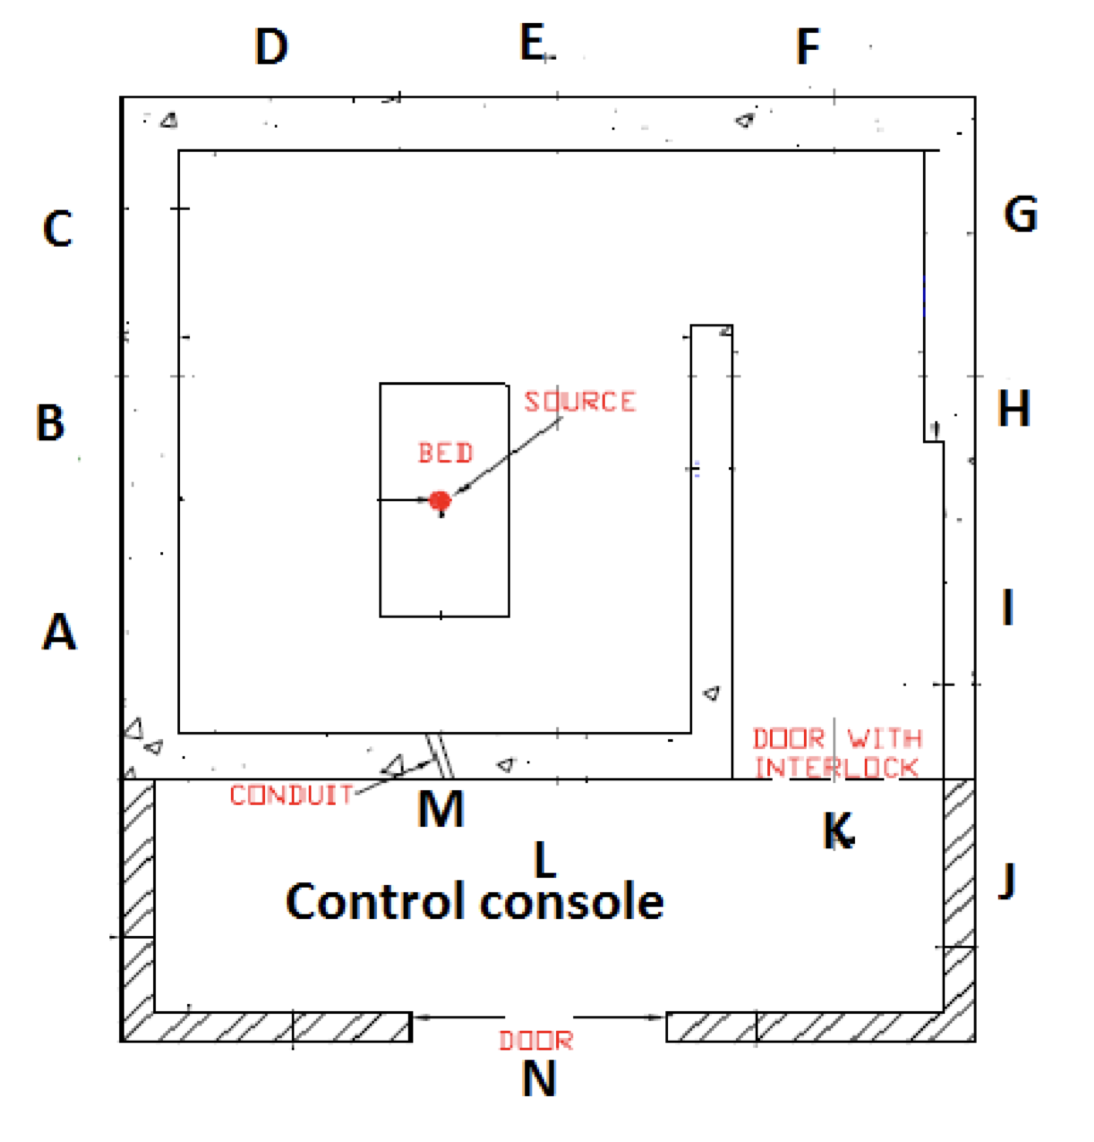
\includegraphics[width=0.4\textwidth]{Figures/Experimental data/LayoutofBrachy.png}
    \caption{Layout of brachytherapy unit in treatment room}
\end{figure}
\begin{figure}[H]
    \centering
    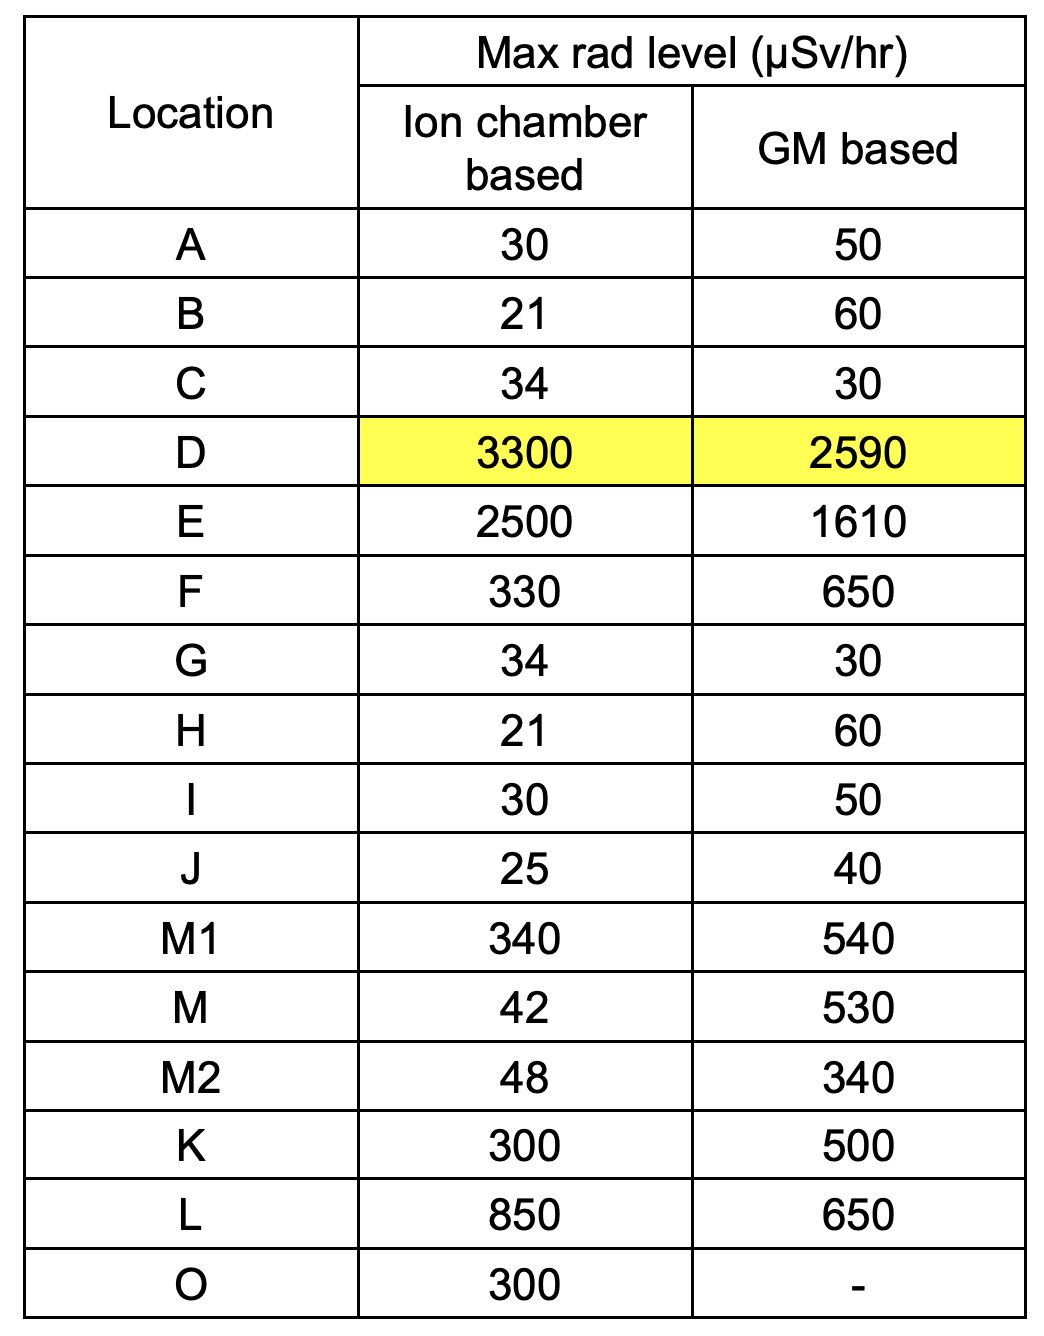
\includegraphics[width=0.6\textwidth]{Figures/Experimental data/Brachydata.png}
\end{figure}

\subsubsection{Weekly Time Averaged Dose-Equivalent Rate}
The weekly time averaged dose-equivalent rate is calculated using the formula,

\begin{equation}
    R_W = \mathrm{IDR} \times \text{weekly treatment time (4 hr/week)} \times \frac{A_0}{A_t}
\end{equation}

\begin{tabular}{ll}
$R_w$ & is the TADR averaged over one week, in $\mathrm{Sv}\cdot\mathrm{week}^{-1}$; \\
IDR & is instantaneous dose-equivalent rate in $\mathrm{Sv}\cdot\mathrm{h}^{-1}$ when the machine is operating at the activity $A_t$; \\
$A_0$ & is the initial activity of the source, in Ci; $= 10 \text{ Ci}$ \\
$A_t$ & is the current activity of the source, in Ci; $= 8.281 \text{ Ci}$ \\
\end{tabular}

\begin{itemize}
    \item For \textbf{ion based survey meter}, $R_w = 3300 \times 10^6 \text{ R/hr}\times 4 \text{ hr/week} \times \frac{10}{8.2} = 0.01609 \text{ R/week}$.
    \item For \textbf{GM based survey meter}, $R_w =  2.59 \times 10^{-3}\text{R/hr}\times 4 \text{ hr/week} \times \frac{10}{8.2} = 0.01263 \text{ R/week}$.
\end{itemize}


